\documentclass[tikz]{standalone}
\usetikzlibrary{cd}

\newcommand{\id}{\mathrm{id}}
\newcommand{\C}{\mathcal{C}}
\newcommand{\D}{\mathcal{D}}

\begin{document}
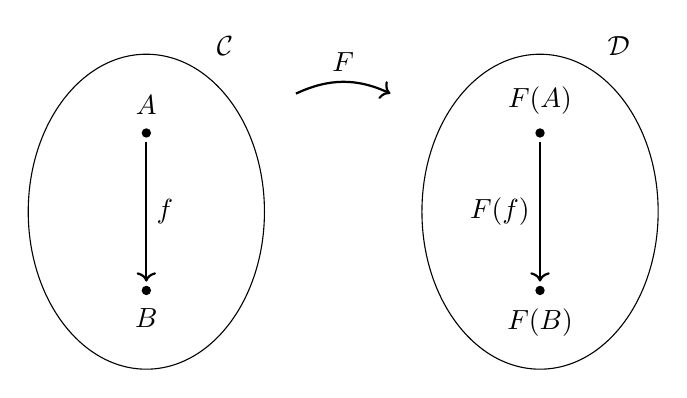
\begin{tikzpicture}
    % Catégorie C
    \draw (2,2) ellipse (1.5cm and 2cm);
    \node(C) at (3,4.1) {$\C$};

    \draw (2,3) node[circle, inner sep=1.2pt, outer sep=1.5pt, fill=black, label={above:{$A$}}] (A) {};
    \draw (2,1) node[circle, inner sep=1.2pt, outer sep=1.5pt, fill=black, label={below:{$B$}}] (B) {};
    \draw [thick, ->] (A) -- node[right] {$f$} (B);

    % Catégorie D
    \draw (7,2) ellipse (1.5cm and 2cm);
    \node(D) at (8,4.1) {$\D$};
    \draw (7,3) node[circle, inner sep=1.2pt, outer sep=1.5pt, fill=black, label={above:{$F(A)$}}] (FA) {};
    \draw (7,1) node[circle, inner sep=1.2pt, outer sep=1.5pt, fill=black, label={below:{$F(B)$}}] (FB) {};
    \draw [thick, ->] (FA) -- node[left] {$F(f)$} (FB);

    % Foncteur
    \draw [thick, ->] (3.9,3.5) to [bend left=25] node[above] {$F$} (5.1,3.5);
\end{tikzpicture}
\end{document}
